\documentclass[landscape,a0paper,fontscale=0.292]{baposter}

\usepackage[vlined]{algorithm2e}
\usepackage{times}
\usepackage{calc}
\usepackage{url}
\usepackage{graphicx}
\usepackage{amsmath}
\usepackage{amssymb}
\usepackage{relsize}
\usepackage{multirow}
\usepackage{booktabs}
\usepackage{graphicx}
\usepackage{multicol}
\usepackage[T1]{fontenc}
\usepackage{ae}

\graphicspath{{images/}}

 % Format 
 \newcommand{\RotUP}[1]{\begin{sideways}#1\end{sideways}}

 % Multicol Settings
 \setlength{\columnsep}{0.7em}
 \setlength{\columnseprule}{0mm}

  % Save space in lists. Use this after the opening of the list
 \newcommand{\compresslist}{%
 \setlength{\itemsep}{1pt}%
 \setlength{\parskip}{0pt}%
 \setlength{\parsep}{0pt}%
 }

%\definecolor{NUpurpleNormal}{rgb}{.321,0,.388}
\definecolor{NUpurpleDark}{rgb}{.221,0,.288}
\definecolor{NUpurpleLite}{rgb}{.553,0,.720}


%%%%%%%%%%%%%%%%%%%%%%%%%%%%%%%%%%%%%%%%%%%%%%%%%
\begin{document}

\begin{poster}{
 % Show grid to help with alignment
 grid=false,
 % Column spacing
 colspacing=0.7em,
 % Color style
 bgColorOne=white,
 bgColorTwo=white,
 borderColor=NUpurpleLite,
 headerColorOne=NUpurpleDark,
 headerColorTwo=NUpurpleLite,
 headerFontColor=white,
 boxColorOne=white,
 boxColorTwo=NUpurpleLite,
 % Format of textbox
 textborder=roundedleft,
 % Format of text header
 eyecatcher=true,
 headerborder=closed,
 headerheight=0.1\textheight,
%  textfont=\sc, An example of changing the text font
 headershape=roundedright,
 headershade=shadelr,
 headerheight=0.12\textheight}
 % Eye Catcher
 {
     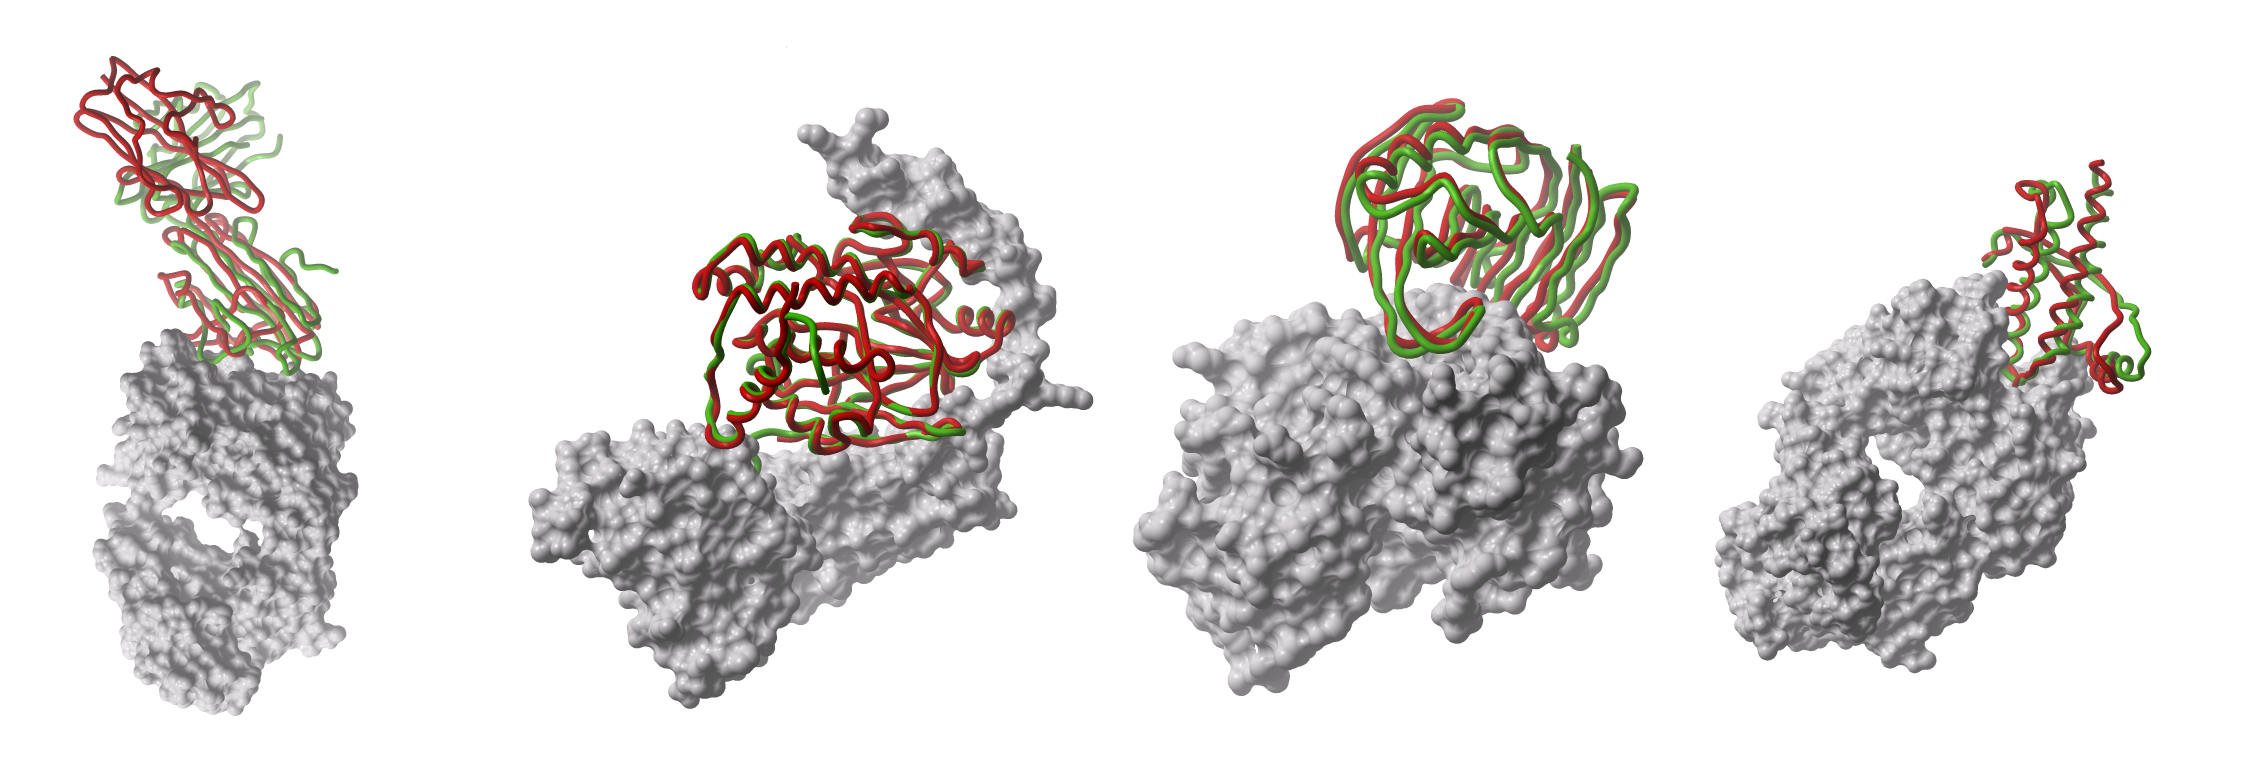
\includegraphics[width=0.23\linewidth]{protein-eyecatcher3fixed.png}
 }
 % Title
 {\sc\huge Predicting Protein-Protein Interaction via SVM Learning }
 % Authors
 {Charleston Noble and Alex Zylman\\[0.5em]
 {\texttt{\large charlestonnoble2012@u.northwestern.edu, azylman@u.northwestern.edu\\}}
 {\texttt{\large Northwestern University, EECS 349: Machine Learning, Dr. Bryan Pardo}}}
 % University logo
 {
  \begin{tabular}{r}
    
\includegraphics[height=0.10\textheight]{logo2.png}\\
  \end{tabular}
 }


%%%%%%%%%%%%%%%%%%%%%%%%%%%%%%%%%%%%%%%%%%%%%%%%%%%%%%%%%%%%%%%%%%%%%%%%%%%%%%
  \headerbox{Contribution: Classification From \emph{PRIMARY} Structure}{name=contribution,column=0,row=0,span=2}{
%%%%%%%%%%%%%%%%%%%%%%%%%%%%%%%%%%%%%%%%%%%%%%%%%%%%%%%%%%%%%%%%%%%%%%%%%%%%%%
 Interactions between proteins are essential for the large majority of biological functions, so predicting whether two proteins will interact is a central problem in medical and biological research. We propose a method which accomplishes this task with only the most basic knowledge of the two proteins: their primary structures.
  }


%%%%%%%%%%%%%%%%%%%%%%%%%%%%%%%%%%%%%%%%%%%%%%%%%%%%%%%%%%%%%%%%%%%%%%%%%%%%%%
  \headerbox{Protein Structure}{name=abstract,column=0,below=contribution}{
%%%%%%%%%%%%%%%%%%%%%%%%%%%%%%%%%%%%%%%%%%%%%%%%%%%%%%%%%%%%%%%%%%%%%%%%%%%%%%
 Proteins are linear chains of \emph{amino acids}, which fold to form complex three dimensional structures. 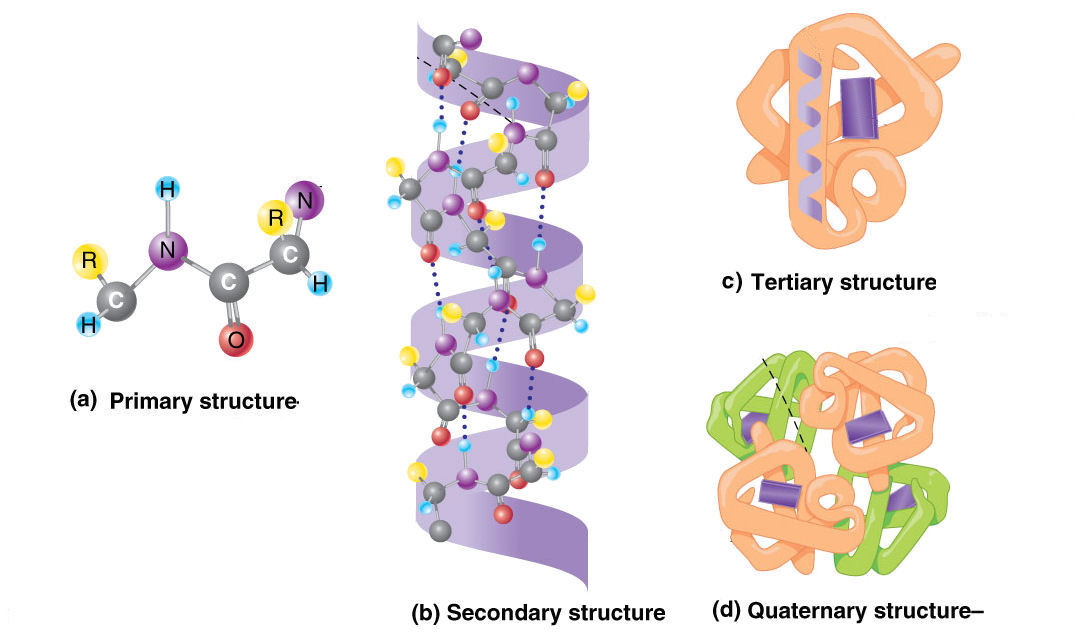
\includegraphics[width=1.0\linewidth]{protein_structure_fixed.jpg} A protein's \emph{primary structure} is simply its amino acid sequence, while secondary, tertiary and quaternary structures refer to its local and global three dimensional shape.
}


 %%%%%%%%%%%%%%%%%%%%%%%%%%%%%%%%%%%%%%%%%%%%%%%%%%%%%%%%%%%%%%%%%%%%%%%%%%%%%%
   \headerbox{Support Vector Learning}{name=speed,column=2,row=0,span=2}{
 %%%%%%%%%%%%%%%%%%%%%%%%%%%%%%%%%%%%%%%%%%%%%%%%%%%%%%%%%%%%%%%%%%%%%%%%%%%%%%
 Proteins were represented by feature vectors by aggregating descriptors of their amino acid constituents. The descriptors we considered were hydrophobicity, hydrophicility, volumes of side chains, polarity, polarizability, solvent-accessible surface area (SASA) and net charge index (NCI). These descriptors were chosen because they, in particular, affect the binding properties of the overall protein. Aggregate descriptor values for proteins were assembled by finding the autocovariance (AC) of their values up to a distance $lg$ away from a particular amino acid. Given a protein sequence, AC variables describe the average interactions between residues, a certain $lag$ apart throughout the whole sequence. These values were calculated according to:
\begin{equation}
AC_{lag,j}=\frac{1}{n-lag}\sum_{i=1}^{n-lag}\left[\left( X_{i,j}-\frac{1}{n}\sum_{i=1}^{n}X_{i,j}\right)
	\times \left( X_{(i+lag),j}-\frac{1}{n}\sum_{i=1}^{n}X_{i,j}\right)\right]
\end{equation}
where $j$ represents one descriptor, $i$ the position in the sequence $X$, $n$ the length of the sequence $X$ and $lag\leq lg$ the value of the $lag$. The software SVM-Light was employed in the classification of feature vectors. A linear function was chosen as the kernel function due to time constraints. Leave-one-out cross validation was performed.

}


%%%%%%%%%%%%%%%%%%%%%%%%%%%%%%%%%%%%%%%%%%%%%%%%%%%%%%%%%%%%%%%%%%%%%%%%%%%%%%
  \headerbox{References}{name=references,column=0,above=bottom}{ %%%%%%%%%%%%%%%%%%%%%%%%%%%%%%%%%%%%%%%%%%%%%%%%%%%%%%%%%%%%%%%%%%%%%%%%%%%%%
     \smaller
     
     \bibliographystyle{ieee}
     \renewcommand{\section}[2]{\vskip 0.05em}
       \begin{thebibliography}{1}\itemsep=-0.01em
       \setlength{\baselineskip}{0.4em}

       \bibitem{BnG}
        J. R. Bock and D. A. Gough. Predicting protein-protein
	interactions from primary structure. \emph{Bioinformatics},
	17(5).

       \end{thebibliography}
   }


 %%%%%%%%%%%%%%%%%%%%%%%%%%%%%%%%%%%%%%%%%%%%%%%%%%%%%%%%%%%%%%%%%%%%%%%%%%%%%%
   \headerbox{Training + Testing Data}{name=data,column=0,above=references,below=abstract}{
 %%%%%%%%%%%%%%%%%%%%%%%%%%%%%%%%%%%%%%%%%%%%%%%%%%%%%%%%%%%%%%%%%%%%%%%%%%%%%%
 Primary structures of interacting protein pairs were obtained from UCLA's Database of Interacting Proteins which contains over 50000 entries representing pairs of proteins known to mutually bind. Negative interactions were not included in the database, so synthetic native-like pairs were created by permuting sequences of interacting pairs. This permutation was performed using Shufflet, a bioinformatics application developed by Eivind Coward, University of Bergen. All data and source code can be found at: \mbox{\small \url{http://github.com/azylman/Protein-Interactions}} Overall, 134,550 protein-pairs were used, with half of these being interacting pairs and the other half non-interacting.
   }


 %%%%%%%%%%%%%%%%%%%%%%%%%%%%%%%%%%%%%%%%%%%%%%%%%%%%%%%%%%%%%%%%%%%%%%%%%%%%%%

   \headerbox{Results and Optimization}{name=tracking,column=2,span=2,below=speed,above=bottom}{
 %%%%%%%%%%%%%%%%%%%%%%%%%%%%%%%%%%%%%%%%%%%%%%%%%%%%%%%%%%%%%%%%%%%%%%%%%%%%%%
We achieved a 72.56\% accuracy rate using a linear kernel and the full set of features. This compares to the roughly 80\% accuracy of current research into this problem. From there, we wanted to find out which acid descriptors had the largest effect in determining the accuracy of our classifier.\\
Initially, we ran our classifier seven times, each time using all of the descriptors except for one. This way, we get an average accuracy of 72.07\% (with a standard deviation of .31\%), only slightly less than our accuracy using all of the descriptors. The removal of SASA had the largest effect, dropping our accuracy to 71.67\%, while the removal of polarizability had the least effect, dropping our accuracy to 72.46\%.\\
Subsequently, we ran our classifier seven times, each using only one of our seven descriptors. The average accuracy of 61.84\% with a standard deviation of 4.79\%. The descriptor that had the least effect on accuracy was NCI, which had an accuracy of 57.04\%. The descriptor that had the largest effect was polarity, which had an accuracy of 68.08\%. While most of our training was done with a linear kernel, we ran this training data a second time using a radial basis kernel function, which increased our accuracy to 71.4\%.\\
 \begin{center}	 
 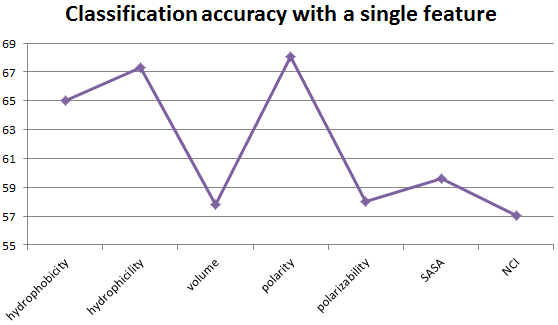
\includegraphics[width=0.35\linewidth]{accuracy.png}
 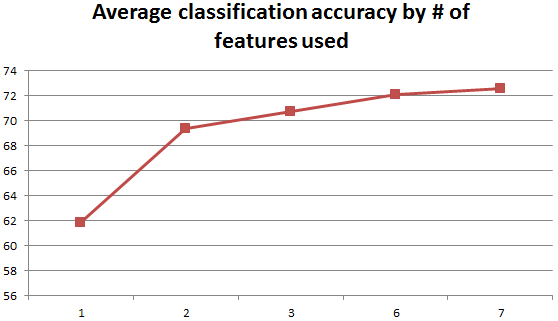
\includegraphics[width=0.35\linewidth]{accuracy-by-num-features.png}
 \end{center}
Next, we wanted to see which descriptor, when paired with polarity, gave the highest accuracy so we ran our classifier six times using each of the remaining six descriptors and polarity. We got an average accuracy of 69.32\% with a standard deviation of .38\%. The descriptor that had the highest accuracy when paired with polarity was SASA at 69.88\%, while the descriptor with the lowest accuracy was 68.92\%.\\
When we look at our descriptors paired with polarity and SASA, the average is 70.67\% and the standard deviation is .46\%. The maximum accuracy of 71.47\% was achieved using volume, polarity, and SASA while the lowest accuracy of 70.36\% was a result of using polarity, SASA, and NCI.
   }

 %%%%%%%%%%%%%%%%%%%%%%%%%%%%%%%%%%%%%%%%%%%%%%%%%%%%%%%%%%%%%%%%%%%%%%%%%%%%%%
   \headerbox{Predicting Interactions}{name=lowrestracking,column=1,above=bottom}{
 %%%%%%%%%%%%%%%%%%%%%%%%%%%%%%%%%%%%%%%%%%%%%%%%%%%%%%%%%%%%%%%%%%%%%%%%%%%%%%
 While the interaction (or non-interaction) status of protein-pairs is determined by their three dimensional shapes, the problem of accurately predicting the shape of  novel proteins remains an open (and enormously complex) problem in bioinformatics. Thus it has been suggested that, since a protein's primary structure determines its tertiary structure, or three dimensional shape, we can skip the intermediate and intractable step of determining the proteins' tertiary structure when attempting to predict interactions. \cite{BnG}
   }


 %%%%%%%%%%%%%%%%%%%%%%%%%%%%%%%%%%%%%%%%%%%%%%%%%%%%%%%%%%%%%%%%%%%%%%%%%%%%%%%
  \headerbox{Protein-Protein Interaction}{name=algorithm,column=1,above=lowrestracking,below=contribution}{
 %%%%%%%%%%%%%%%%%%%%%%%%%%%%%%%%%%%%%%%%%%%%%%%%%%%%%%%%%%%%%%%%%%%%%%%%%%%%%%%
 If two proteins come into contact with each other, and their structures
 complement each other in some region, then they can \emph{bind}, or
 \emph{dock} with each other.
 \begin{center}	 
 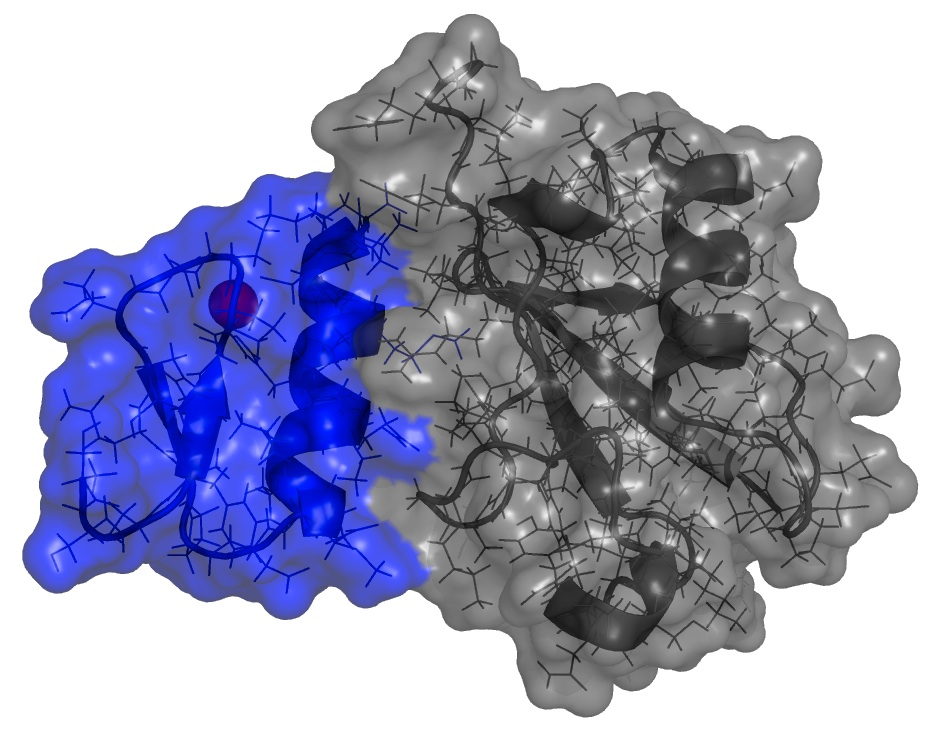
\includegraphics[width=0.8\linewidth]{docking.jpg}
 \end{center}
 If two proteins are capable of binding with each other, then they are said to \emph{interact}. Binding interactions ubiquitous in biological processes, and much of contemporary pharmaceutical research is concerned with the creation of novel interacting proteins. For example, Alzheimer's Disease is thought to be caused by the accumulation of misfolded proteins in the brain, and one proposed cure is the creation of a protein which can interact with these and properly re-orient them.
   }
\end{poster}%
%
\end{document}
